\begin{document}

\def\title{Homework 2}
% \config{hwnum}{2}
% \config{homework-due}{02/0/2019 23:59}
% \config{grades-due}{02/XX/2019 23:59}

\newcommand{\qitem}{\qpart\item}

\renewcommand{\labelenumi}{(\alph{enumi})} % change default enum format to (a)
\renewcommand{\theenumi}{(\alph{enumi})} % fix reference format accordingly.
\renewcommand{\labelenumii}{\roman{enumii}.} % second level labels.
\renewcommand{\theenumii}{\roman{enumii}.}

\maketitle
% \vspace{0.5em}
% {\textbf{Due date:} 2/8/19, at 23:59. Please \LaTeX of handwrite your homework solution and submit an electronic version on Gradescope.}

% {\textbf{Self-grades due date:} 2/XX/19, at 23:59.}

% {\parindent 0pt
% \begin{tabular}[t]{l}
% EECS 127 / EE 227AT \\
% G. Ranade, A. Bayen
% \end{tabular}  \hfill 2/1/19\vskip 0.2in }

% \parindent 0pt
% \parskip 8pt

% \begin{center}
% \large\bf Homework Assignment \#2
% \end{center}

% \bigskip

\noindent
{\bf Release date:}  9/12/19 \\
{\bf Due date:}  9/19/19, 23:00 (11 pm)

Please \LaTeX{} or handwrite your homework solution and submit an electronic version.

\textbf{Submission Format} \\
Your homework submission should consist of a single PDF file that contains all of your answers (any handwritten answers should be scanned) as well as your IPython notebook saved as a PDF.
			
If you do not attach a PDF ``printout'' of your IPython notebook, you will not receive credit for problems that involve coding. Make sure that your results and your plots are visible. Assign the IPython printout to the correct problem(s) on Gradescope.
% \textbf{Submission Format} \\
% Your homework submission should consist of \textbf{two} files.
% \begin{itemize}
% 	\item \verb|hw2.pdf|: A single PDF file that contains all of your answers (any handwritten answers should be scanned) 
% 	as well as your IPython notebook saved as a PDF.
			
% 	If you do not attach a PDF ``printout'' of your IPython notebook, you will not receive credit for problems that involve coding. Make sure that your results and your plots are visible. Assign the IPython printout to the correct problem(s) on Gradescope.
		
% 	\item \verb|hw2.ipynb|: A single IPython notebook with all of your code in it.
% \end{itemize}
% Submit each file to its respective assignment on Gradescope.

\begin{qunlist}
\qns{Vectors and Orthogonality}


Let $\{ v_1,...,v_n\}$ be an orthonormal basis in $\mathbb{R}^n$. Prove for all $x \in \mathbb{R}^n$ that
    \begin{align*}
        \sum_{i=1}^n | \langle x, v_i \rangle |^2 = \langle x,x \rangle.
    \end{align*}

\sol{\item $g(x_1,x_2) = \dfrac{x_1^2}{4} + \dfrac{x_2^2}{9}$


}

\newpage
\qns{Image Representation}

% \todo[inline]{Make sure the symmetries x-axis and y-axis are clearly defined.}
Please refer to the corresponding Jupyter notebook: ``image\_representation.ipynb''
\newpage
\qns{Representation of a graph as a matrix: the adjacency matrix}
% \todo[inline]{Better explain the notations, refer to the definition of the notations.}

In this exercise, we are interpreting a graph as a matrix. 
Then, we show that finding a path between two nodes can be done with a matrix multiplication.  
This can be useful to quickly compute several shortest paths, or to re-compute shortest paths when the weights on the links of the graph only change slightly.

We are given a graph as a set of vertices $V = \{1,...,n\}$, with edges $E \subseteq V \times V$. We assume that the graph is undirected (without arrows), meaning that $(i,j)\in E$ implies $(j,i)\in E$.

We define the adjacency matrix of the graph $A$ by:
\[
A_{ij} = \left\{ 
\begin{array}{ll}
1 & \mbox{if } (i,j) \in E, \\
0 & \mbox{otherwise.}
\end{array}
\right.
\]

\begin{figure}[h]
\centering
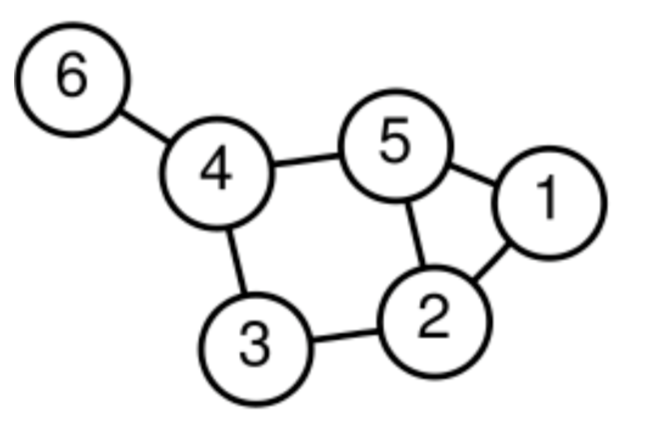
\includegraphics[width=.4\textwidth]{figures/UndirectedGraph.png}
\caption[Graph example]{Example of an undirected graph.}
\label{fig:symm-graph}
\end{figure}

\begin{enumerate}
\item Form the adjacency matrix for the graph shown in Figure~\ref{fig:symm-graph}.

\sol{\item $g(x_1,x_2) = \dfrac{x_1^2}{4} + \dfrac{x_2^2}{9}$


}
\item Turning to a generic graph, show that the adjacency matrix $A$ is symmetric.

\sol{\item Show that the following inequalities hold for any vector $x \in \Real{n}$:
\[
% \|x\|_\infty \le \|x\|_1 \le n \|x\|_\infty \\
% \|x\|_2 \le \|x\|_1 \le \sqrt{n} \|x\|_2 \\
% \|x\|_\infty \le \|x\|_2 \le\sqrt{n}\|x\|_\infty \\
\frac{1}{\sqrt{n}}\|x\|_2 \leq \|x\|_\infty \leq  \|x\|_2 \leq \|x\|_1 \leq \sqrt{n} \|x\|_2 \le n\|x\|_\infty.
\]

\textit{Hint:} For $\|x\|_1\leq \sqrt{n}\|x\|_2$, how might you express $\|x\|_1$ as the dot product of two vectors? Can you then use the Cauchy-Schwarz inequality to bound this dot product?}
\end{enumerate}

Now let's show that if there is a path between $i\in V$ and $j\in V$, then there exists $n\in \mathbb{N}$ such that $e_i^\top A^n e_j \neq 0$. We define $e_i$ as the vector of length $n$ where the $i$th entry is $1$ and all other entries are $0$. 

Let's proceed by induction. Define the following property:
\begin{align}
    P(n) : \text{ there is a path of length } n \text{ between } i \text{ and } j \implies e_i^\top A^n e_j \neq 0
\end{align}


And show that $P(1)$ is true and that $\forall n>1,\ P(n-1)\implies P(n)$. This will show that $\forall n\geq 1$, $P(n)$ is true.

% Formally the length $n$ of a path $p$ is the number of edges that it contains.

To get some intuition about the exercise that you will now solve, it is strongly recommended to run the iPython notebook ``Adjacency matrix.ipynb''.
You do \textbf{NOT} need to submit the iPython notebook to gradescope.

Let assume that there is a path -- denoted $p$ -- between $i$ and $j$. We denote the length of the path $p$ as $n$.

\begin{enumerate}
\setcounter{enumi}{2}
\item Show that if $n=1$ -- meaning that there is a path of length $1$ between $i$ and $j$ -- then $e_i^\top A^n e_j \neq 0$. State what is the value of $e_i^\top A^n e_j$.

\sol{\item $g(x) = \sin(x_1^2) \log (x_3 - x_2)$ where $x_i$ are scalars and $x_3 - x_2 > 0$.}
\end{enumerate}

Now let's assume that the property is true for $n-1$, with $n>1$. Let show that it is true for $n$.

\begin{enumerate}
\setcounter{enumi}{3}
\item Show that $e_i^\top A^n e_j = \sum\limits_k (e_i^\top A e_k) (e_k^\top A^{n-1} e_j)$.
This equation means that any path of length $n$ between $i$ and $j$ is the combination of a link between $i$ and a vertices $k$ and a path of length $n-1$ from $k$ to $j$.

\sol{\item
\[
g(x) = \begin{bmatrix}
x_1^2/x_2 \\
\log(x_3) \sin(x_1/x_3)
\end{bmatrix}
\]}
\item Show that $\forall k, (e_i^\top A e_k) (e_k^\top A^{n-1} e_j)\geq 0$.

\sol{\input{adjacency_solutions/5}}
\end{enumerate}

Let's denote $l$ the first node achieved in the path $p$ from $i$.

\begin{enumerate}
\setcounter{enumi}{5}
\item Explain why $e_l^\top A^{n-1} e_j \neq 0$.

\sol{\input{adjacency_solutions/6}}
\item State the value of $e_i^\top A e_l$.

\sol{\input{adjacency_solutions/7}}
\item Conclude that $e_i^\top A^n e_j \neq 0$.

\sol{\input{adjacency_solutions/8}}
\item Have you shown that there is a path between $i$ and $j$ if and only if $e_i^\top A^n e_j\neq 0$ ?

\sol{\input{adjacency_solutions/9}}

If you enjoyed this exercise, feel free to read:
\begin{itemize}
    \item Algebraic Graph Theory, C.Godsil, G.Royle
    \item Algebraic Graph Algorithms, P.Sankowski
\end{itemize}

\end{enumerate}
\newpage
\qns{Gram-Schmidt}
\newline
Any set of $n$ linearly independent vectors in $\mathbb R^n$ could be used as a basis for $\mathbb R^n$. However, certain bases could be more suitable for certain operations than others. For example, an orthonormal basis could facilitate solving linear equations.

\begin{enumerate}

\item Given a matrix $A \in \mathbb R^{n \times n}$, it could be represented as a multiplication of two matrices
\[ A = Q R, \]
where $Q$ is a unitary matrix (its columns form an orthonormal basis for $\mathbb R^n$) and $R$ is an upper-triangular matrix. For the matrix $A$, describe how Gram-Schmidt process could be used to find the $Q$ and $R$ matrices, and apply this to 
\[ A = 
\begin{bmatrix} 3 & -3 & 1\\
4 & -4 & -7 \\
0 & 3 & 3
\end{bmatrix}
\] 
to find a unitary matrix $Q$ and an upper-triangular matrix $R$.

\sol{\item $g(x_1,x_2) = \dfrac{x_1^2}{4} + \dfrac{x_2^2}{9}$


}

\item Given an invertible matrix $A \in \mathbb R^{n \times n}$ and an observation vector $b \in \mathbb R^n$, the solution to the equality
 \[ A x = b \]
is given as $x = A^{-1}b$. For the matrix $A = QR$ from part (a), assume that we want to solve
\[ A x = \begin{bmatrix}
8 \\ -6 \\ 3
\end{bmatrix}. \]
By using the fact that $Q$ is a unitary matrix, find $\overline b$ such that
\[ R x = \overline b. \]

Then, given the upper-triangular matrix $R$ and $\overline b$ in part (c), find the elements of $x$ \underline{sequentially}.

\sol{\item Show that the following inequalities hold for any vector $x \in \Real{n}$:
\[
% \|x\|_\infty \le \|x\|_1 \le n \|x\|_\infty \\
% \|x\|_2 \le \|x\|_1 \le \sqrt{n} \|x\|_2 \\
% \|x\|_\infty \le \|x\|_2 \le\sqrt{n}\|x\|_\infty \\
\frac{1}{\sqrt{n}}\|x\|_2 \leq \|x\|_\infty \leq  \|x\|_2 \leq \|x\|_1 \leq \sqrt{n} \|x\|_2 \le n\|x\|_\infty.
\]

\textit{Hint:} For $\|x\|_1\leq \sqrt{n}\|x\|_2$, how might you express $\|x\|_1$ as the dot product of two vectors? Can you then use the Cauchy-Schwarz inequality to bound this dot product?}

\item Describe how your solution in the previous problem is akin to Gaussian elimination in solving a system of linear equations.

\sol{\item $g(x) = \sin(x_1^2) \log (x_3 - x_2)$ where $x_i$ are scalars and $x_3 - x_2 > 0$.}

\item Given an invertible matrix $B \in \mathbb R^{n \times n}$ and an observation vector $c \in \mathbb R^n$, find the computational cost of finding the solution $z$ to the equation $Bz = c$ by using the $QR$ decomposition of $B$. Assume that $Q$ and $R$ matrices are available, and adding, multiplying, and dividing scalars take one unit of ``computation". 

As an example, computing the inner product $a\tran b$ is said to be $O(n)$, since we have $n$ scalar multiplications total -- one for each $a_i b_i$. Similarly, matrix vector multiplication is $O(n^2)$, since matrix vector multiplication can be viewed as computing $n$ inner products. The computational cost for inverting a matrix in $\mathbb R^n$ is $O(n^3)$, and consequently, the cost grows rapidly as the set of equations grows in size. This is why the expression $A^{-1}b$ is usually not computed by directly inverting the matrix $A$. Instead, the $QR$ decomposition of $A$ is exploited to decrease the computational cost.

\sol{\item
\[
g(x) = \begin{bmatrix}
x_1^2/x_2 \\
\log(x_3) \sin(x_1/x_3)
\end{bmatrix}
\]}

\end{enumerate}

\end{qunlist}
\end{document}
